\documentclass[
	12pt,				% tamanho da fonte
	openany,			% capítulos começam em pág ímpar (insere página vazia caso preciso)
	oneside, 			% oneside - twoside
	a4paper,			% tamanho do papel.
	chapter=TITLE,		% títulos de capítulos convertidos em letras maiúsculas
	section=TITLE,		% títulos de seções convertidos em letras maiúsculas
	sumario=tradicional,	
	%subsection=TITLE,	% títulos de subseções convertidos em letras maiúsculas
	%subsubsection=TITLE,% títulos de subsubseções convertidos em letras maiúsculas
	english,			% idioma adicional para hifenização
	brazil,				% o último idioma é o principal do documento
	]{abntex2}

% User commands
\usepackage{xcolor}
\newcommand\myworries[1]{\textcolor{red}{[#1]}}

% Pacotes fundamentais
\usepackage{lmodern}
%\usepackage{helvet}			% Usa a fonte Latin Modern
%\renewcommand{\familydefault}{\sfdefault} tira o serifado
\usepackage[T1]{fontenc}		% Selecao de codigos de fonte.
\usepackage[utf8]{inputenc}		% Codificacao do documento (conversão automática dos acentos)
\usepackage{indentfirst}		% Indenta o primeiro parágrafo de cada seção.
\usepackage{color}				% Controle das cores
\usepackage{tikz}				% Inclusão de gráficos
\usepackage{graphicx}			% Inclusão de gráficos
\usepackage{microtype} 			% para melhorias de justificação
% Pacotes adicionais, usados no anexo do modelo de folha de identificação
\usepackage{multicol}
\usepackage{multirow}
% Pacotes adicionais, usados apenas no âmbito do Modelo Canônico do abnteX2
\usepackage{lipsum}				% para geração de dummy text
% Pacotes de citações
\usepackage[brazilian,hyperpageref]{backref}	 % Paginas com as citações na bibl
\usepackage[alf,abnt-etal-list=3,abnt-etal-cite=3]{abntex2cite}	% Citações padrão ABNT
\usepackage{pdflscape}
\usepackage{listings}			% inserir codigo fonte
\usepackage{footnote}
\usepackage{pdfpages}
\usepackage{caption}

% [leolleo] meus pacotes
\usepackage{booktabs}
\usepackage{adjustbox}
\usepackage{subcaption}
\usepackage[labelfont=bf]{caption}
\usepackage{gensymb}
\usepackage{amsmath}
\usepackage{array}
\usepackage{float}
\usepackage{xcolor,colortbl}
\usepackage{longtable}
\usepackage{scalefnt}
% [leolleo] meus comandos (peguei do tex exchange)

\usepackage{tocloft}
% -- permite a adição de células especiais em tabelas
\newcommand{\specialcell}[2][c]{%
  \begin{tabular}[#1]{@{}c@{}}#2\end{tabular}}

\newcounter{equationset}
\newcommand{\equationset}[1]{% \equationset{<caption>}
  \refstepcounter{equationset}% Step counter
  \noindent\makebox[\linewidth]{Equação ~\theequationset: #1}
 }

\renewcommand{\ABNTEXchapterfont}{\fontseries{b}}
\renewcommand{\ABNTEXchapterfontsize}{\normalsize}

\renewcommand{\ABNTEXsectionfont}{\fontseries{m}}
\renewcommand{\ABNTEXsectionfontsize}{\normalsize}

\renewcommand{\ABNTEXsubsectionfont}{\fontseries{b}}
\renewcommand{\ABNTEXsubsectionfontsize}{\normalsize}

\renewcommand{\ABNTEXsubsubsectionfont}{\fontseries{m}}
\renewcommand{\ABNTEXsubsubsectionfontsize}{\normalsize}

%-------

% CONFIGURAÇÕES DE PACOTES
% Configurações do pacote backref
% Usado sem a opção hyperpageref de backref
\renewcommand{\backrefpagesname}{Citado na(s) página(s):~}
% Texto padrão antes do número das páginas
\renewcommand{\backref}{}
% Define os textos da citação
\renewcommand*{\backrefalt}[4]{
	\ifcase #1 %
		%Nenhuma citação no texto.%
	\or
		Citado na página #2.%
	\else
		Citado #1 vezes nas páginas #2.%
	\fi}%


% Configurações de aparência do PDF final
% alterando o aspecto da cor azul
\definecolor{blue}{RGB}{41,5,195}
% informações do PDF
\makeatletter
\hypersetup{
     	%pagebackref=true,
		pdftitle={\@title},
		pdfauthor={\@author},
    	pdfsubject={\imprimirpreambulo},
	    pdfcreator={LaTeX with abnTeX2},
		pdfkeywords={abnt}{latex}{abntex}{abntex2}{relatório técnico},
		colorlinks=true,			% false: boxed links; true: colored links
    	linkcolor=black,				% color of internal links
    	citecolor=black,				% color of links to bibliography
    	filecolor=black,			% color of file links
		urlcolor=black,
		bookmarksdepth=4
}
\makeatother
% ---

% ---
% Espaçamentos entre linhas e parágrafos
% ---

% O tamanho do parágrafo é dado por:
\setlength{\parindent}{1.3cm}

% Controle do espaçamento entre um parágrafo e outro:
\setlength{\parskip}{0.2cm}  % tente também \onelineskip

% ---
% compila o indice
% ---
\makeindex
% ---


\newcommand{\imagem}[4]
{%			\imagem{x.x}{nomeimg}{titulo}{fonte}
	\begin{figure}[!htb]
		\caption{\label{img:#2}#3}
		\begin{center}
			\includegraphics[scale=#1]{img/#2}
		\end{center}
        \legend{\textbf{Fonte:} #4}
	\end{figure}
}%

\newcommand{\xx} {$\bigotimes$}
\newcommand{\oo} {$\bigcirc$}

 % Comandos Essenciais

\titulo{SISTEMA DE INFORMAÇÃO ONLINE PARA LEITURA E ARMAZENAMENTO DE DADOS METEOROLÓGICOS}
\autor{GABRIEL RAFAEL GOMES}
\local{JUAZEIRO - BA}
\orientador{Prof. M. Sc. Fábio Nelson de Sousa Pereira}
%\coorientador{M. Sc. Osvaldo Campelo de Mello Vasconselos}
\instituicao{
UNIVERSIDADE FEDERAL DO VALE DO SÃO FRANCISCO
	\par
CURSO DE GRADUAÇÃO EM ENGENHARIA DE COMPUTAÇÃO}
\tipotrabalho{Trabalho de Conclusão de Curso}
\preambulo{Trabalho apresentado à Universidade Federal do Vale do São Francisco - Univasf, Campus Juazeiro, como requisito da obtenção do título de Bacharel em Engenharia de Computação.}

%%%%% Início do TCC %%%%%%

% CONFIGURACAO DO SUMARIO
% -----------------------------------------------------------------------------
% Secao primaria (Chapter) Caixa alta, Negrito, tamanho 12
\makeatletter
\renewcommand*{\l@chapter}[2]{%
  \l@chapapp{\uppercase{#1}}{#2}{\cftchaptername}}
\makeatother
% Secao secundaria (Section) Caixa baixa, Negrito, tamanho 12
\renewcommand{\cftsectionfont}{\uppercase} %ponha \rmfamily se quiser serifadas...

% Secao terciaria (Subsection) Caixa baixa, negrito, tamanho 12
\renewcommand{\cftsubsectionfont}{\bfseries}

% Secao quaternaria (Subsubsection) Caixa baixa, tamanho 12
\renewcommand{\cftsubsubsectionfont}{\normalfont}

% Seção quinaria (subsubsubsection) Caixa baixa, sem negrito, tamanho 12
\renewcommand{\cftparagraphfont}{\normalfont\itshape}


\begin{document}

	\frenchspacing % Retira espaço extra obsoleto entre as frases.
	\pretextual
		\begin{capa}
\center
	
\includegraphics[scale=0.6]{img/univasf.jpg}

	{\ABNTEXchapterfont\bfseries\large\imprimirinstituicao}

	\vspace*{5cm}
	{\ABNTEXchapterfont\bfseries\large\imprimirautor}

	\vfill
	{\ABNTEXchapterfont\bfseries\large\imprimirtitulo}
	\vfill
	\ABNTEXchapterfont\bfseries\large\imprimirlocal\\ \the\year

	\vspace*{1cm}

\end{capa}

\begin{folhaderosto}
\center
		{\ABNTEXchapterfont\bfseries\large\imprimirautor}
		\vspace*{\fill}

		{\ABNTEXchapterfont\bfseries\large\imprimirtitulo}
		\vspace*{\fill}

		{\hspace{.45\textwidth}
		\begin{minipage}{.5\textwidth}
			\SingleSpacing
			\imprimirpreambulo \\ \\

			{\imprimirorientadorRotulo~\imprimirorientador\par}
			{\imprimircoorientadorRotulo~\imprimircoorientador\par}

		\end{minipage}%
		\vspace*{\fill}}%
		\vspace*{\fill}
			\ABNTEXchapterfont\bfseries\large\imprimirlocal\\ \the\year
		\vspace*{1cm}
\end{folhaderosto}


%\begin{fichacatalografica}
%	\vspace*{\fill}					% Posição vertical
%	\hrule							% Linha horizontal
%	\begin{center}					% Minipage Centralizado
%	\begin{minipage}[c]{12.5cm}		% Largura
%
%	\imprimirautor
%
%	\hspace{0.5cm} \imprimirtitulo  / \imprimirautor. --
%	\imprimirlocal, \the\year-
%
%	\hspace{0.5cm} xx p. : il. (algumas color.) ; 30 cm.\\
%
%	\hspace{0.5cm} \imprimirorientadorRotulo~\imprimirorientador\\
%
%	\hspace{0.5cm}
%	\parbox[t]{\textwidth}{\imprimirtipotrabalho~--~\imprimirinstituicao,
%	\the\year.}\\
%
%	\hspace{0.5cm}
%		1. Palavra-chave1.
%		2. Palavra-chave2.
%		I. Orientador.
%		II. Universidade xxx.
%		III. Faculdade de xxx.
%		IV. Título\\
%
%	\hspace{8.75cm} CDU 02:141:005.7\\
%
%	\end{minipage}
%	\end{center}
%	\hrule
%\end{fichacatalografica}

\setlength{\ABNTEXsignwidth}{12cm}
\begin{folhadeaprovacao}
	\begin{center}
	    {\ABNTEXchapterfont\bfseries\large\imprimirinstituicao}
	    \vspace*{\fill}

	    {\ABNTEXchapterfont\bfseries\large FOLHA DE APROVAÇÃO}
	    \vspace*{\fill}

	    {\ABNTEXchapterfont\bfseries\large\imprimirautor}

	    \vspace*{\fill}\vspace*{\fill}
	    {\ABNTEXchapterfont\bfseries\large\imprimirtitulo}
	    \vspace*{\fill}

	    {\hspace{.45\textwidth}
		\begin{minipage}{.5\textwidth}
			\SingleSpacing
			\ABNTEXchapterfont\imprimirpreambulo \\ \\

			{\ABNTEXchapterfont\imprimirorientadorRotulo~\imprimirorientador\par}
			{\ABNTEXchapterfont\imprimircoorientadorRotulo~\imprimircoorientador\par}

		\end{minipage}%
	    \vspace*{\fill}}
	\end{center}

	\vspace*{\fill}	
	
	\begin{center}
			 \ABNTEXchapterfont\large Aprovado em: \_\_\_\_ de \_\_\_\_ de 2017
	\end{center}

	\vspace*{\fill}
	
	\begin{center}
			 \ABNTEXchapterfont\bfseries\large Banca Examinadora
	\end{center}
		
   \ABNTEXchapterfont\assinatura{Fábio Nelson de Sousa Pereira, Mestre, Universidade Federal do Vale do São Francisco}
	\ABNTEXchapterfont\assinatura{Jorge Luis Cavalcanti Ramos, Doutor, Universidade Federal do vale do São Francisco}
   \ABNTEXchapterfont\assinatura{Ricardo Argenton Ramos, Doutor, Universidade Federal do Vale do São Francisco}
	 \vspace*{\fill}

	 
\end{folhadeaprovacao}

% -- epígrafe
\newpage
\vspace*{\fill}
\begin{flushright}
		\textit{A minha família...}
\end{flushright}

\begin{agradecimentos}
	
	A minha mãe Josiane Gomes, meu pai Weliton de Carvalho e meus irmãos pelo esforço imensurável para que minha formação se concretizasse.
	
	Ao meu primo Manoel Rafael pelo apoio essencial durante a vida acadêmica.
	
	Aos meus amigos e companheiros de turma pela parceria, colaboração, compartilhamento de estresse e de fortes emoções durante o curso. Especialmente Esron Dtamar, Johnathan Alves, Gustavo Marques e Leonardo Cavalcante.
	
	Aos amigos conquistados no decorrer da caminhada, João Bastos, José Matias, Delmiro Daladier, Daniel Simião, Hallan Ferreira, Victor Silva, Antônio Noronha, Marlon Rocha e o pessoal restante do grupo do "AP" pela partilha da tarimba, casos e contos em mesas de bar.
	
	A Ana Letícia Menezes pelo companheirismo, paciência e pelo abraço caloroso.
	
	A meu tio Antônio Marcos pelo exemplo integridade e competência no aspecto pessoal e profissional.
	
	A meu primo Marco Antônio pela inspiração e minha tia Neiva Gomes por toda educação e amor dados à mim.
	
	Ao meu orientador, professor Fábio Nelson, pelos ensinamentos, dedicação e disposição.
	
	Aos professores Rômulo Câmara e Jairson Rodrigues pelas oportunidades de trabalhos extracurriculares que me enriqueceram muito como pessoa e profissional.
	
	A todos os demais professores que repassaram para mim um pouco de seu conhecimento e experiência, contribuindo de alguma forma para a realização deste trabalho e para minha formação.
	
	A minha madrinha Lúcia Ricarte, Joelma Duarte e Lurdinéia Guimarães por todo carinho e apoio de sempre.

	Por fim, agradeço a todos aqueles que auxiliaram de alguma maneira a existência e o desenvolvimento de meu ser.

\end{agradecimentos}

% ---
% Epígrafe
% ---
\begin{epigrafe}
    \vspace*{\fill}
	\begin{flushright}
		Se pude enxergar a tão grande distância, foi subindo nos ombros de gigantes.\\
		 \vspace{\baselineskip}
		\textbf{Isaac Newton}\\
		\textbf{Carta à Robert Hooke, 1676}
	\end{flushright}
\end{epigrafe}
% ---


% ---
% RESUMOS
% ---
% resumo em português
\setlength{\absparsep}{18pt} % ajusta o espaçamento dos parágrafos do resumo
\begin{resumo}
	Na região do Submédio do Vale do São Francisco, a organização social Biofábrica Moscamed Brasil, ou simplesmente Moscamed, sediada na cidade de Juazeiro-BA, é responsável pelo controle biológico da mosca-das-frutas e do mosquito-da-dengue. Esta é uma das maiores regiões produtoras de frutas do mundo. Entretanto, diversas culturas são atacadas pela praga da mosca-das-frutas ocasionando perdas consideráveis na produção. Por outro lado, a Moscamed atua também no combate ao mosquito \textit{Aedes Aegypti}, que é vetor de diversas doenças de grande importância quando se diz respeito à saúde pública. A Moscamed emprega um dos métodos mais eficazes no controle de ambos os insetos, a Técnica do Inseto Estéril (TIE). Porém, os ciclos de vida das duas espécies e consequentemente o êxito da técnica citada estão fortemente relacionados com as alterações climáticas do ambiente. Deste modo, visando auxiliar a tomada de decisões no que diz respeito aos processos relacionado à TIE e os demais processos da organização, o presente trabalho tem o intuito de desenvolver um sistema de informação  \textit{web}/aplicativo \textit{Android} que fornece um mecanismo de obtenção e armazenamento e uma interface de visualização dos dados das variáveis climáticas provenientes de uma estação meteorológica \textit{Vantage Vue \textsuperscript{TM}}.

 \textbf{Palavras-chave}: \textit{Vantage Vue, Android, Ionic, Weather Link IP}, meteorologia.

\end{resumo}

% resumo em inglês
\begin{resumo}[Abstract]
\begin{otherlanguage*}{english}

	In the sub-region of the São Francisco Valley, the social organization Biofábrica Moscamed Brasil, or simply Moscamed, based in the city of Juazeiro-BA, is responsible for the biological control of the medfly and the dengue mosquito. This is one of the largest fruit producing regions in the world. However, several crops are attacked by the medfly pests, causing considerable losses in production. On the other hand, the Aedes Aegypti mosquito, which is a vector of several diseases of great importance when it comes to public health. Moscamed employs one of the most effective methods in controlling both insects, the Sterile Insect Technique (TIE). However, the life cycles of both species and consequently the success of the cited technique are strongly related to the environmental changes of the environment. In this way, in order to assist in the decision making process related to TIE and other processes of the organization, the present work aims to develop an information system that provides a retrieval and storage mechanism and a visualization interface of weather data from a Vantage Vue\textsuperscript{TM} weather station. The work was done using web technologies, framework for multiplatform applications and non relational database. The resulting system consists of a web / Android application as the user interface, an application that retrieves weather station information and an API to manage the data.
	
	\vspace{\onelineskip}

	\noindent
	\textbf{Key-words}: \textit{Vantage Vue, Android, Ionic, Weather Link IP, meteorology}.

 \end{otherlanguage*}
\end{resumo}


% ---
% inserir lista de ilustrações
% ---
\begin{KeepFromToc}
\pdfbookmark[0]{\listfigurename}{lof}
\listoffigures
%\addcontentsline{toc}{chapter}{Lista de Figuras}
\cleardoublepage


% ---
% inserir lista de tabelas
% ---
\pdfbookmark[0]{\listtablename}{lot}
\listoftables
\cleardoublepage

% ---
\end{KeepFromToc}
% inserir lista de abreviaturas e siglas
% ---
\begin{siglas}
	\item[API]      \textit{Application programming interface} - tradução: Interface de programação de aplicativos
    \item[APP]		\textit{Application} - tradução: Aplicação
	\item[ART]      \textit{Android runtime} - tradução: Tempo de execução \textit{Android}
	\item[CECOMP]	Colegiado de engenharia de computação
	\item[CSS]      \textit{Cascading style sheet} - tradução: Tabela de estilos em cascata
    \item[GNU]		\textit{Gnu's not unix} - tradução: Gnu não é Unix
	\item[HAL]      \textit{Hardware abstration layer} - tradução: Camada de abstração de \textit{hardware} 
	\item[HTML]     \textit{Hypertext markup language} - tradução: Linguagem  de marcação de hipertexto
	\item[HTTP]     \textit{Hypertext transfer protocol} - tradução: Protocolo de transferência de hipertexto
	\item[IDE]      \textit{Integrated development environment} - tradução: Ambiente de desenvolvimento integrado
	\item[INMET]	Instituto nacional de meteorologia
    \item[JSON]	    \textit{Javascript object notation} - tradução: Notação de objeto Javascript
	\item[MIP]      Manejo integrado de pragas
    \item[MIT]		\textit{Massachusetts institute of technology} - tradução: Instituto de tecnologia de Massachusetts
	\item[REST]     \textit{Representational state transfer} - tradução: Transferência de Estado Representacional
	\item[SDK]		\textit{Software development kit} - tradução: Kit de desenvolvimento de programa
	\item[SGBD]		Sistema de gerenciamento de banco de dados
	\item[TCC]      Trabalho de conclusão de curso
    \item[TCP]		\textit{Transfer control protocol} - tradução: Protocolo de controle de transmissão 
	\item[TIE]		Técnica do inseto estéril
	\item[UR]	    Umidade relativa
	\item[URI]	    \textit{Uniform resource identifier} - tradução: Identificador de recurso univeforme
	\item[XML]      \textit{Extensible markup language} - tradução: Linguagem de marcação extensível
    
\end{siglas}

\pdfbookmark[0]{\contentsname}{toc} % inserir o sumario
\tableofcontents*
\cleardoublepage


	\textual
		\pagestyle{simple}
		\chapter{Introdução}

A mosca-das-frutas é uma praga causadora de diversos danos à produção de frutas e hortaliças. No Submédio do Vale do São Francisco são encontradas várias espécies desses insetos. A Organização Moscamed Brasil surge com a intenção de realizar a supressão dessa população através da Técnica do Inseto Estéril - TIE, cuja aplicação é adotada em mais de 28 países \cite{MOSCAMEDINST2003}. 

Além da mosca-das-frutas, a Moscamed também é responsável pelo controle biológico da espécie de mosquito \textit{Aedes Aegypti}, vetor da doença reemergente mais importante do mundo, a dengue. Quando em 2007 cerca de 70\% dos Municípios brasileiros estavam infestados pelo mosquito \cite{BRAGA2007}. Neste caso, o controle ocorre de forma análoga ao das moscas, ambos usufruem da TIE.

A técnica criada por E.F.Knipling consiste em produzir machos estéreis e liberá-los na natureza em grande quantidade. As fêmeas da natureza então copulam com os machos estéreis e colocam ovos não fecundados, fazendo com que a próxima geração tenha sua densidade populacional reduzida \cite{paranhos2008moscas}. O êxito da TIE depende do sucesso dos machos estéreis na competição contra os nativos pelo acasalamento com as fêmeas da mosca-das-frutas ou do mosquito-da-dengue, e da consequente postura dos ovos não fecundados.

Contudo, o ciclo de vida das moscas na natureza é fortemente dependente da temperatura ambiente, além de outros fatores climáticos \cite{raga2000manejo}. A mosca-da-carambola necessita, por exemplo, de vinte e dois dias com clima favorável (26 ºC e 70\% UR) para se desenvolver completamente partindo da fase de ovo até a fase adulta \cite{malavasi2000moscas}. De mesmo modo, o ciclo de vida dos mosquitos também é fortemente dependente da temperatura e de outros fatores climáticos, seja em seu desenvolvimento ou em sua sobrevivência \cite{hopp2001global, ribeiro2006associaccao}.

Neste contexto, com a finalidade de auxiliar a organização em suas tomadas de decisão, a proposta deste TCC é composta pelo desenvolvimento de um sistema \textit{Web}/aplicativo \textit{Android open-source} para consulta e armazenamento em banco de dados de informações provenientes de uma estação meteorológica sem fio \textit{Vantage Vue \textsuperscript{TM}}, instalada na Biofábrica Moscamed Brasil.

\section{Justificativa}

Este TCC é um subprojeto do projeto Sistema de Gestão da Produção de Insetos Modificados para Regiões Endêmicas, conjunto entre a Moscamed e o Colegiado de Engenharia de Computação da Universidade Federal do Vale do São Francisco - CECOMP.


\section{Objetivos gerais}

Desenvolver um sistema capaz de informar, via \textit{internet}, dados meteorológicos obtidos de uma estação \textit{Vantage Vue \textsuperscript{TM}} e disponibilizar para o usuário dados e gráficos através de uma aplicação \textit{Web} e de um aplicativo para o sistema operacional \textit{Android}.

\section{Objetivos específicos}

\begin{itemize}
    \item Modelar graficamente a arquitetura do sistema por meio de diagramas de casos de uso, diagrama de atividades, diagrama de sequência e protótipos das telas de interface com o usuário;
    \item Definir a melhor forma de estruturar os dados provenientes da estação meteorológica;
    \item Modelar a API responsável por armazenar e disponibilizar os dados;
	\item Desenvolver a versão inicial do sistema.
\end{itemize}

\section{Organização do trabalho}

O trabalho é dividido em três seções, fundamentação teórica, metodologia e conclusão e trabalhos futuros.

A fundamentação teórica é organizada em duas subseções, na primeira é explanado sobre a Moscamed, suas responsabilidades e a técnica de controle biológico empregada. Em seguida é estudada a estação meteorológica em questão e a influência das variáveis climáticas nas espécies controladas pela Moscamed. A segunda parte discorre sobre as bases conceituais das tecnologias utilizadas no processo de desenvolvimento, como a pilha de software do sistema operacional \textit{Android}, desenvolvimento \textit{web} e desenvolvimento de aplicações \textit{cross-platform}.

Na metodologia são estudadas os passos para a concepção e construção do sistema através de diagramas e modelos gráficos dos seus vários elementos, como por exemplo banco de dados e interface de usuário. Nesse capítulo, ainda é mostrado o conjunto de tecnologias adotadas para a implementação do sistema.    

No capítulo de resultados e discussões é apresentada uma descrição detalhada das funcionalidades do sistema desenvolvido.

O capítulo conclusão e trabalhos futuros mostra sucintamente os resultados obtidos com a finalização do projeto e algumas sugestões que podem ser realizadas a posteriori.

		\chapter{Referencial teórico}

\section{Moscamed, a instituição e a técnica}

A Biofábrica Moscamed Brasil é uma organização social situada no Vale do São Francisco, mais precisamente em Juazeiro-BA, responsável pelo controle biológico e monitoramento ambientalmente seguro de pragas em culturas de alto interesse econômico, tais como, manga, uva, melão, maçã, papaia, goiaba e acerola \cite{MOSCAMED2010LINHAS}. Bem como o controle do vetor transmissor de doenças mais importante para a saúde pública atualmente, o mosquito \textit{Aedes Aegypt} \cite{MOSCAMEDINST2003, MOSCAMED2010LINHAS}.

A organização possui atividades em larga escala voltadas para a produção e liberação na natureza de insetos estéreis modificados, via raios-X no caso da mosca-das-frutas e via alteração genética no caso do Mosquito-da-dengue. Possui o planejamento de produção/liberação de 200 (duzentos) milhões de machos estéreis por semana \cite{MOSCAMEDINST2003, MOSCAMED2003CTI}. Ademais, realiza capacitação, treinamento e disseminação de informações técnico-científicas de sua área de atuação para a comunidade \cite{MOSCAMED2010AREAS}.

O controle e monitoramento é realizado através da TIE em ambas as linhas de produção. Concebida em 1937, por Edward F. Knipling, a TIE é considerada um tipo de controle autocida ou genético, visto que a praga é utilizada em seu próprio controle \cite{TIE2015}. Os insetos estéreis são produzidos e liberados em quantidades bem maiores do que as encontradas na natureza, competem pelo acasalamento com os selvagens e acabam copulando com as fêmeas. As fêmeas, por sua vez, no caso das moscas, realizam a postura de ovos não fecundados. Já no caso dos mosquitos, o gene modificado repassado para as próximas gerações elimina ou inviabiliza as fêmeas adultas. As duas maneiras fazem com que a geração posterior de insetos tenha sua população reduzida. A repetição deste processo continuamente garante a manutenção do baixo índice populacional e em alguns casos leva à erradicação \cite{MOSCAMEDINST2003, MOSCAMED2003CTI, MOSCAMED2010LINHAS}.

Segundo \citeonline{TIE2015}, até 1970 o controle de insetos era efetuado por meio de métodos baseados na utilização de inseticidas químicos sintéticos. O uso dos inseticidas sofreu diversas restrições durante a década de 70, à partir de então popularizou-se o conceito de Manejo Integrado de Pragas (MIP), onde diferentes ferramentas de controle (como por exemplo produtos químicos, agentes biológicos, ferômonios, dentre outras) são integradas de maneira planejada e coerente. A TIE foi posteriormente incorporada aos programas de MIP em grandes áreas, pois se trata de uma técnica de controle biológico onde as ações não são diretamente executadas por um produtor e sim por uma coordenação regional gestora do programa. A TIE supre, em sua maioria, a necessidade de tratamento com inseticidas no combate às pragas, promovendo a redução das despesas de produção e o aumento consequente da qualidade final e da segurança alimentar do produto agrícola \cite{MOSCAMED2003CTI}.

Cerca de 28 países estão aplicando a TIE em larga escala para supressão populacional e erradicação em locais como a Ásia, ilhas do Pacífico, Oceania, África, Europa e alguns países das Américas e Caribe. No Brasil, 11 estados são beneficiados pela TIE por intermédio da coordenação da Moscamed juntamente ao Ministério da Agricultura, Pecuária e Abastecimento e das Agências estaduais de Defesa Agropecuária. São os estados da Bahia, Pernambuco, Ceará, Rio Grande do Norte, Piauí, Paraíba, Sergipe, Minas Gerais, Espírito Santo, Rio Grande do Sul e Santa Catarina \cite{MOSCAMEDINST2003, MOSCAMED2003CTI}.


\section{A estação meteorológica e a influência das condições climáticas nas espécies controladas pela Moscamed}

As estações meteorológicas surgiram com a finalidade de suprir a necessidade de medir variáveis climáticas. O estudo dessas variáveis é de grande valia para as atividades humanas, pois implica de forma direta ou indireta no atual modelo de desenvolvimento, visto que uma política de desenvolvimento sustentável necessita de monitoramento sobre os recursos naturais finitos fortemente relacionados ao clima. No Brasil, inicialmente, a obtenção e avaliação de dados meteorológicos coletados era feita por intermédio do Instituto Nacional de Meteorologia - INMET. Esse processo possuía uma amostragem relativamente pequena e estava sujeita à erros humanos \cite{torres2015aquisicao}.
  
O crescimento tecnológico proporcionou a possibilidade da criação de estações meteorológicas automáticas que abrem mão da interferência humana, prevenindo assim a ocorrência de erros e além disso incrementam consideravelmente o desempenho, praticidade e confiabilidade das medições realizadas \cite{torres2015aquisicao}.  

A estação meteorológica \textit{Vantage Vue™} (figura \ref{img:estacao}) é uma estação automática \textit{wireless} composta de dois módulos, sendo o primeiro deles um conjunto de sensores (figura \ref{img:sensores}) e o segundo um console (figura \ref{img:console}). A suíte de sensores é alimentada por energia solar, inclui uma bateria reserva e contém os seguintes sensores: coletor de chuva, sensor de umidade/temperatura, anemômetro e sensor de direção do vento. Após a coleta de dados pelos sensores, os mesmos são atualizados e enviados via rádio de baixa potência para o console \cite{SITEDAVIS, VVINSTMANUAL}.

\newpage

\begin{figure}[!htb]
\centering
    \caption{\label{img:estacao} A estação meteorológica \textit{Vantage Vue™}}
    \subcaptionbox{\label{img:sensores} Suíte de sensores}{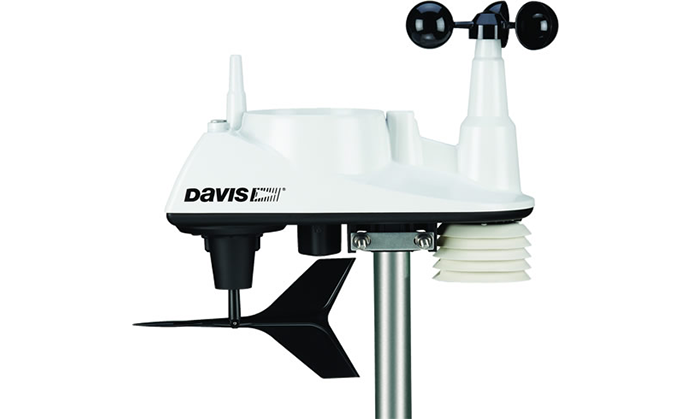
\includegraphics[scale=.26]{img/vantagevue}}\qquad
    \subcaptionbox{\label{img:console} Console}
{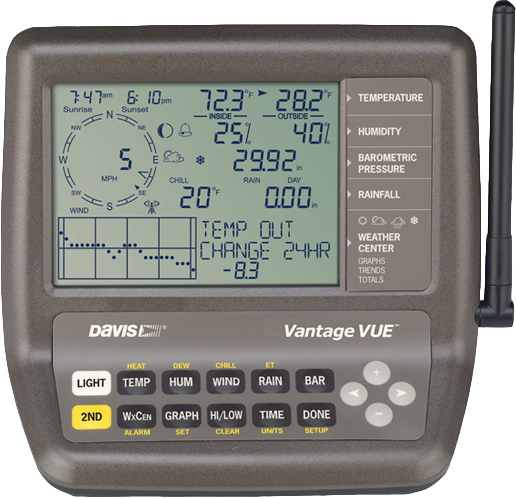
\includegraphics[scale=.21]{img/console}}
    \legend{\textbf{Fonte:} \citeonline{SITEDAVIS}}
\label{fig:dag}
\end{figure}

Por sua vez, o console \textit{Vantage Vue™} é responsável pela exibição e registro dos dados de sua estação. Possui também a opção de interação com computador via módulo \textit{ethernet} vendido separadamente, \textit{WeatherLinkIP}® (figura \ref{img:weatherlinkip}) \cite{SITEDAVIS, VVCINSTMANUAL}.

\imagem{0.57}{weatherlinkip}{O \textit{datalogger WeatherLinkIP®}}{O autor}
\newpage

O módulo \textit{WeatherLinkIP}® consiste de um \textit{datalogger} que conecta o console da estação à internet. O módulo transfere os dados climáticos obtidos do console para o computador, com a finalidade gerar uma base de dados permanente. As principais variáveis exportadas e arquivadas pelo \textit{datalogger} são a hora/data da medição, temperatura interna e externa, direção e velocidade do vento, precipitação e a umidade interna e externa \cite{WLIP}.

O tamanho da memória não volátil do módulo é de 128KB. A memória é preenchida de acordo com o intervalo (em minutos) de atualização definido pelo usuário. Portanto, o período de tempo ao qual as amostras se referem pode ter uma extensão maior ou menor. Por exemplo, caso o usuário escolha a taxa de atualização de um e um minuto, o módulo terá espaço suficiente para armazenar dados de cerca de quarenta e duas horas. Por outro lado, se a frequência de atualização for de trinta minutos, o armazenamento terá dados de cinquenta e três dias \cite{WLIP}.

\subsection{A influência do clima na mosca-das-frutas}

A mosca-das-frutas é um inseto que sofre diversas alterações em seu ciclo de vida de acordo com as mudanças climáticas. Por volta de 250 (duzentas e cinquenta) espécies dessas pragas atacam variedades de plantas frutíferas de grande interesse econômico. São insetos da ordem \textit{Diptera} e família \textit{Tephritidae}. Estão presentes em todo território brasileiro, porém existem dois gêneros com importância maior, sendo uma originária das Américas Central e do Sul e outra cuja a introdução no país ocorreu no início do século XX, os gêneros \textit{Anastrepha} e \textit{Ceratitis}, respectivamente. Na Região do Vale do Submédio São Francisco há 11 (onze) espécies de \textit{Anastrepha} já identificadas \cite{paranhos2008moscas}.

Os ciclos de vida de ambos os gêneros supracitados são semelhantes, diferencia\-ndo-se apenas na questão do tempo de desenvolvimento das fases. O ciclo se inicia com a oviposição realizada pela fêmea nos frutos, após a eclosão a larva penetra no endocarpo e depois deixam o fruto para empupar no solo e por fim emergirem como adultos \cite{paranhos2008moscas}.
  
Segundo \citeonline{calore2013fatores}, em um estudo relacionado aos insetos de goiaba, a sazonalidade dos elementos climáticos/meteorológicos têm influência direta ou indireta sobre esses insetos. Diretamente, os elementos do clima podem atuar na mortalidade ou no desenvolvimento dos insetos, alterando a oviposição, alimentação, crescimento, desenvolvimento e migração. Os aspectos climáticos podem atuar de forma indireta pela influência na atividade dos inimigos naturais dos insetos e pela variação na qualidade dos recursos disponíveis devido as mudanças fisiológicas e bioquímicas na planta hospedeira.

Ainda de acordo com \citeonline{calore2013fatores}, as variáveis meteorológicas que estão mais relacionadas com a dinâmica populacional de insetos e diversos ecossistemas são a temperatura, a umidade relativa, a precipitação pluviométrica e a velocidade do vento. Em algumas espécies a evaporação, a insolação e o fotoperíodo também são importantes.

Em relação a mosca-das-frutas têm-se a temperatura do ar como principal influenciador no desenvolvimento de suas fases de ovo, larva e adulta, enquanto a temperatura do solo é predominante na fase de pupa \cite{garcia1998influencia}. Por exemplo, em situações de temperaturas superiores a 35ºC ou inferiores a 10ºC não há desenvolvimento de nenhuma das fases do ciclo de vida da mosca-da-fruta da espécie \textit{Anastrepha fraterculus} \cite{araujo2008levantamento}. Além disso, em regiões semiáridas a precipitação, as temperaturas elevadas e a disponibilidade de hospedeiros regem os picos populacionais da mosca-das-frutas da espécie citada, pois a precipitação ocasiona o aumento da umidade no solo, viabilizando o desenvolvimento da fase de pupa, que em sua maioria ocorre numa camada contemplada pelos dez primeiros centímetros do solo. Essa camada é altamente vulnerável ao dessecamento e portanto pode causar a inviabilidade das pupas e dificultar a emergência dos adultos devido ao solo ressecado \cite{calore2013fatores, araujo2008levantamento}.

\subsection{A influência do clima no mosquito-da-dengue}

De forma análoga à mosca-das-frutas, os mosquitos \textit{Aedes Aegypti} também sofrem variações em seu ciclo vital e em seu comportamento mediante modificações climáticas. De acordo com \citeonline{hopp2001global}, o aumento da temperatura global e outras mudanças climáticas podem modificar a área geográfica de presença desse inseto. Como por exemplo na Colômbia, onde os insetos eram limitados pela altitude de 1500 metros devido ao intenso frio e hoje em dia são encontrados em níveis acima de 2200 metros em razão da elevação da temperatura.
 
A temperatura e a precipitação pluviométrica, apresentam grande significância em relação ao desenvolvimento e sobrevivência dessa espécie, como pode ser observado na figura \ref{img:aedeslc} \cite{hopp2001global, ribeiro2006associaccao}. 

Ainda na figura \ref{img:aedeslc}, em algumas fases estão destacadas as faixas de valores das variáveis que são cruciais para o desenvolvimento e/ou sobrevivência do inseto, em outras etapas destaca-se apenas a dependência de determinados fatores. Na incubação por exemplo (transição entre a fase de ovo e a fase de larva), necessita-se da temperatura igual ou superior a 13ºC e uma lâmina d’água de pelo menos 10 milímetros de espessura. Em outro caso, na fase de pupa o desenvolvimento do inseto é sensível à temperatura média diária. As faixas de temperaturas aqui ilustradas são referentes à taxa de sobrevivência igual a 1 (um), como pode ser visualizado na figura \ref{img:survivor}.

%\newpage

\imagem{0.54}{aedeslc}{O Ciclo de Vida do Mosquito \textit{Aedes Aegypti} e suas dependências climáticas diárias}{\citeonline{hopp2001global} (Adaptado) }
 
\imagem{0.55}{survivor}{Dependência da temperatura na sobrevivência dos estágios de vida do mosquito \textit{Aedes Aegypti}}{\citeonline{hopp2001global}(Adaptado) }

De acordo com \citeonline{depradine2004climatological}, uma elevada pressão de vapor de água facilita a atividade dos mosquitos, tornando suas atividades de alimentação ou ataque mais frequentes, provocando a propagação acentuada da doença.

Além do ciclo de vida do mosquito, a dinâmica de casos de doenças relacionadas ao vetor também flutua com as condições do clima. A flutuação está diretamente ligada ao aumento de temperatura, pluviosidade e umidade do ar, pois o conjunto desses fatores favorecem o crescimento da quantidade de criadouros disponíveis e o desenvolvimento do vetor \cite{ribeiro2006associaccao}.

\section{Sistema Operacional Android}

O \textit{Android} é a plataforma de desenvolvimento \textit{mobile} mais popular do mundo, está presente em mais de 190 países e possui centenas de milhões de dispositivos ativos. A plataforma conta com a contribuição da comunidade \textit{open-source} Linux e mais de 300 parceiros em \textit{hardware}, \textit{software} e operadoras. A plataforma permite a criação de aplicativos por meio da linguagem de programação Java. A Google, dententora da plataforma, disponibiliza o Kit de Desenvolvimento de Software (\textit{Software Development Kit - SDK}) e o Ambiente de Desenvolvimento Integrado (IDE) para a criação de aplicativos nativos para \textit{Android} \cite{SITEANDROID}.

\subsection{Características e Arquitetura}

A pilha de software da plataforma \textit{Android} possui código aberto e é baseada em Linux, conforme ilustrada pela figura \ref{img:Android2}. A escolha do Linux como base da pilha é justificada pela utilização de recursos de segurança, outras atividades de gerenciamento de \textit{hardware} já disponíveis nesse sistema operacional e pela facilidade proporcionada aos fabricantes no desenvolvimento de \textit{drivers} de \textit{hardware} para um \textit{kernel} conhecido \cite{SITEANDROID, gandhewar2010google}.

\imagem{0.72}{Android2}{A pilha de software do Android}{\citeonline{SITEANDROID2} (Traduzido)}

A segunda camada, abstração de \textit{hardware} (\textit{Hardware Abstration Layer - HAL}), é responsável por fornecer para a interface de programação de aplicação (\textit{Application Programming Interface - API}) Java o acesso aos componentes de \textit{hardware}, tais como o módulo de câmera ou \textit{bluetooth}. O \textit{Android Runtime - ART} é capaz de executar para cada aplicativo uma máquina virtual própria que requer poucos recursos, possibilitando a execução de vários aplicativos simultaneamente. Os dois últimos componentes e alguns serviços são implementados em código nativo que utiliza bibliotecas em C/C++, porém essas funcionalidades podem ser acessadas através de APIs Java \cite{SITEANDROID}.

O sistema operacional fornece seus recursos por intermédio de APIs programadas em linguagem Java. As APIs compõem os blocos necessários para a criação dos aplicativos, como o sistema de visualização e os gerenciadores de recursos, notificações e atividades \cite{SITEANDROID}.

Na camada mais alta têm-se os aplicativos padrão do sistema que podem ser utilizados para prover funcionalidade à outros aplicativos de terceiros, eliminando a necessidade de desenvolver novamente uma funcionalidade, por exemplo o envio de uma mensagem de texto ou a captura de uma fotografia \cite{SITEANDROID, saha2008developer}.

\section{Aplicações Web}

O grande sucesso da \textit{Web} como arquitetura para desenvolvimento de aplicações pessoais, sociais e de negócios tem impulsionado os desenvolvedores à criarem novas aplicações ou portar \textit{softwares} existentes para a \textit{Web} \cite{fraternali1998conceptual}. A numerosidade das aplicações desenvolvidas fez nascer a necessidade de estabelecer padrões/princípios para o desenvolvimento de aplicações \textit{Web} \cite{pressman2000tangled}.
   
A engenharia de software de desenvolvimento \textit{Web} possui pontos semelhantes e diferentes em relação à de \textit{software} convencionais. É semelhante pelo fato de buscar a realização de uma aplicação correta e completa, mediante os requisitos propostos, e difere porque deve considerar a arquitetura \textit{Web} para sua execução \cite{conte2005processos}.

As aplicações \textit{Web} podem ser divididas em duas categorias, aplicações hipermídia \textit{Web} e aplicações de \textit{software Web}. A primeira é uma aplicação não-convencional onde as informações são disseminadas através de nós, \textit{links}, âncoras, estruturas de acesso e é disponibilizada na \textit{Web}. As tecnologias utilizadas comumente para desenvolver essas aplicações são o \textit{HyperText Markup Language - HTML}, JavaScript e pacotes de multimídia. As aplicações de \textit{software Web} são aplicações nos modelos tradicionais que dependem da arquitetura \textit{Web} para seu funcionamento, tais como sistemas legados de banco de dados, bases de conhecimento, \textit{e-commerce}, entre outros \cite{mendes2005investigating}.

A elaboração de aplicações \textit{Web} deve considerar três dimensões em sua concepção, são elas:

\begin{itemize}
	\item Estrutural: diz respeito a organização das informações e seus relacionamentos semânticos.
	\item Navegacional: como o nome já diz, representa a forma como as informações organizadas pela camada Estrutural serão acessadas.
	\item Apresentação: é a forma como as informações e a aparência dadas à ela serão expostas ao usuário.
\end{itemize}

A qualidade da navegação e da apresentação são tão importantes quanto a qualidade da informação em si \cite{fraternali1998conceptual}. O principal objetivo da engenharia de software \textit{Web} é que haja o desenvolvimento correto da aplicação em termos de estrutura, funcionalidades, aspectos navegacionais e interação com o usuário \cite{pastor2004fitting}.

\section{Aplicações Multiplataformas}

O desenvolvimento de aplicativos multiplataformas consiste em gerar aplicações para diversos sistemas operacionais e para \textit{Web} à partir de um único código fonte. Essa forma de desenvolver ganha mais popularidade à cada dia, principalmente devido ao fato de algumas ferramentas permitirem a utilização de linguagens de programação bastante conhecidas pela comunidade, tais como o HTML, JavaScript e o \textit{Cascading Style Sheet (CSS)}. O código nativo de cada sistema operacional é mascarado por chamadas à APIs, realizadas apenas quando se deseja operar sobre um dispositivo, como câmera ou giroscópio \cite{raj2012study, palmieri2012comparison, dalmasso2013survey}.

Devido ao fato de se possuir apenas uma base de código, a manutenibilidade do software se torna bem menos custosa do que prover soluções nativas específicas para cada plataforma \cite{raj2012study}. \citeonline{palmieri2012comparison} destacam alguns pontos positivos relacionados ao desenvolvimento de aplicações com esse tipo de ferramenta:

\begin{itemize}
\item Redução das habilidades requeridas aos programadores;
\item Redução do tamanho do código;
\item Redução do tempo de desenvolvimento e custos de manutenção a longo prazo;
\item Redução de conhecimento necessário sobre às APIs nativas;
\item Maior facilidade de desenvolvimento;
\item Incremento da participação no mercado.
\end{itemize}


Aplicações \textit{cross-platform} podem ser classificadas em quatro tipos de abordagem, \textit{Web}, Híbrida, Interpretada e Compilação Cruzada. A abordagem \textit{Web} classifica aplicações cuja execução é feita no navegador do dispositivo móvel e os dados são providos por um servidor, neste caso nenhuma instalação é realizada no armazenamento do aparelho. A metodologia Híbrida requer instalação e também usa o navegador do aparelho para renderizar e mostrar as telas da aplicação, porém existe a possibilidade de efetuar chamadas às APIs JavaScript com a finalidade de operar sobre o \textit{hardware} do aparelho \cite{raj2012study, dalmasso2013survey}.

As aplicações interpretadas, como o próprio nome já diz, têm seu código interpretado em tempo de execução por um interpretador. Assim como as aplicações Híbridas, possuem uma camada de abstração que provê o acesso ao \textit{hardware} via APIs. No caso da Compilação Cruzada, o código fonte é convertido para os códigos binários nativos de cada plataforma e o \textit{hardware} é acessado pelas APIs nativas de cada sistema \cite{raj2012study}.

Existem prós e contras em cada tipo de abordagem, portanto deve-se adotar a que mais se adequa ao projeto a ser desenvolvido. Por exemplo, a abordagem \textit{Web} não possui acesso aos sensores do aparelho \textit{mobile}, já a abordagem Híbrida possui performance inferior em relação as aplicações nativas, pois são executadas no navegador. Enquanto isso, na metodologia de Compilação Cruzada, códigos específicos de cada plataforma não podem ser reutilizados, como interface, acesso à localização e notificações \cite{raj2012study}.

A seleção da metodologia ideal depende majoritariamente dos requerimentos da aplicação. A tabela \ref{tab:crossplatform} mostra em uma escala de valores, quais abordagens são ideais para cada tipo de aplicação: 1 – Não preferível, 2 – Preferível, mas não é a metodologia ideal e 3 – Metodologia perfeita \cite{raj2012study}.

\begin{table}[!htb]
	\centering
	\caption{\label{tab:crossplatform} Tipos de aplicações e abordagens preferenciais.}
	\begin{adjustbox}{max width=\textwidth}
		\begin{tabular}{@{} p{5cm} ccc @{}}
		\toprule
		\textbf{Código da Aplicação} & \textbf{Web} & \textbf{Híbrida} & \textbf{Interpretada / Compilação Cruzada} \\ \hline

		\textbf{Aplicações baseadas em dados providos por um servidor} &
			3 & 2 & 1
		\\ \hline

		\textbf{Aplicações independentes} & 1 & 2 & 3\\ \hline

		\textbf{Aplicações baseadas em sensores e processamento de dados no dispositivo} & 1 & 2 & 3\\ \hline

		\textbf{Aplicações baseadas em sensores e processamento de dados no servidor} & 1 & 3 & 2\\ \hline

		\textbf{Aplicações Cliente-Servidor} & 1 & 3 & 2 \\ \bottomrule
	\end{tabular}
	\end{adjustbox}
	\legend{\textbf{Fonte:} \citeonline{raj2012study} (Traduzido)}
\end{table}


\section{API RESTful}
O estilo de arquitetura REST (\textit{Representational State Transfer}) consiste da utilização dos verbos do protocolo HTTP para representar ações no acesso à recursos identificados por um URI (\textit{Uniform Resource Identifier}). As comunicações realizadas com o estilo REST são \textit{stateless}, ou seja, os dados de uma requisição antiga não são repassados para uma requisição posterior. Portanto, é necessário o envio de todas as informações a cada nova requisição. As respostas enviadas pela API ao cliente possuem o formato JSON (\textit{Javascript Object Notation}) ou XML (\textit{Extensible Markup Language}) independentemente da representação original do recurso \cite{arcuri2017restful, fielding2000architectural}.

Os verbos HTTP utilizados comumente nesse tipo de arquitetura são o GET, POST, PUT e DELETE. As aplicações dos verbos estão exemplificadas na tabela \ref{tab:httpverbs} abaixo.

\begin{table}[!htb]
	\centering
	\caption{\label{tab:httpverbs} Métodos HTTP.}
	\begin{adjustbox}{max width=\textwidth}
		\begin{tabular}{@{} p{4cm} c p{10cm} @{}}
		\toprule
		\textbf{Método HTTP} & \textbf{Ação} & \textbf{Notas} \\ \hline

		\textbf{GET} &
			Ler & Recupera um recurso. \newline Exemplo: GET /livros/1 (recupera o recurso de identificador 1) \newline GET /livros (recupera vários recursos) \\ \hline

		\textbf{POST} & Criar & Cria um recurso com os parâmetros repassados. \newline Exemplo: POST /livros {“nomeLivro” : “nome”} 
\\ \hline

		\textbf{PUT} & Atualizar & Atualiza ou cria (caso não exista) um recurso identificado, com os valores repassados. \newline Exemplo: PUT /livros/1 {“nomeLivro” : “novoNome”}
\\ \hline

		\textbf{DELETE} & Deletar & Deleta um recurso identificado. \newline Exemplo: DELETE /livros/1 (deleta o recurso de identificador 1)
 \\ \bottomrule
	\end{tabular}
	\end{adjustbox}
	\legend{\textbf{Fonte:} \citeonline{hsieh2016method} (Traduzido)}
\end{table}

\section{Socket TCP}
O protocolo TCP (\textit{Transmission Control Protocol}) trabalha entregando os pacotes recebidos aos respectivos protocolos de aplicação atribuídos às portas de destino. Por exemplo, ao receber um pacote destinado à porta 80, os dados são entregues ao protocolo HTTP \cite{torres2001completo}.

Porém, quando mais de uma aplicação de mesmo tipo estão comunicando-se com a rede é necessário o uso de um \textit{socket} para definir uma conexão diferente para cada aplicação dentro de uma porta. Os \textit{sockets} gerados quando o transmissor e o receptor criam uma conexão, são definidos em duas classes, ativo e passivo. O primeiro é aquele que envia dados, enquanto o segundo é aquele que recebe dados \cite{torres2001completo}.

As aplicações comunicam-se escrevendo e lendo de seus respectivos \textit{sockets}, ou seja, um \textit{socket} é a interface entre a camada de aplicação e a de transporte dentro de uma máquina como ilustra a figura \ref{img:tcpsocket} \cite{james2005redes}.

\newpage
\imagem{0.75}{tcpsocket}{Processos de aplicação, \textit{sockets} e protocolo de transporte subjacente}{\citeonline{james2005redes}}
		\chapter{Materiais e Métodos} \label{ch:MM}

Este capítulo tem como finalidade descrever o projeto de \textit{software} através da metodologia utilizada, de maneira a elucidar as várias facetas e componentes do sistema como um todo. O capítulo está dividido nas seguintes partes: Projeto de software e Tecnologias utilizadas.

\section{Projeto de Software} 

O projeto foi construído baseando-se em uma adaptação da metodologia Cascata em conjunto com a metodologia Iterativa e Incremental.

A metodologia Cascata foi cunhada por \citeonline{royce1970managing}. É composta por cinco etapas, onde a saída de cada etapa se torna a entrada da etapa posterior. Para isso, é necessário que a etapa anterior seja concluída e esteja correta para que se possa prosseguir com o desenvolvimento. As etapas do modelo são mostradas pela figura \ref{img:cascata}.

\imagem{0.6}{cascata}{Modelo de Desenvolvimento de \textit{Software} Cascata}{\citeonline{royce1970managing} (Traduzido)} 

A primeira etapa busca compreender os requisitos do sistema, que normalmente baseiam-se nas funcionalidades que precisam ser fornecidas, nas limitações e nos objetivos do software. Em seguida há o projeto do sistema, composto do modelo de dados, arquitetura do \textit{software}, interfaces de usuário e demais detalhes \cite{SITECASCATA1, SITECASCATA2}.

As etapas de implementação e testes dizem respeito à programação do \textit{software} em si e ao correto funcionamento das lógicas internas e funcionalidades externas do sistema, respectivamente. Por último têm-se a etapa de operação/manutenção, esta etapa resume-se a implantação, correção de erros não identificados durante a verificação, melhorias funcionais e suporte ao projeto \cite{SITECASCATA1, SITECASCATA2}.

A adaptação buscou simplificar o método cascata para adequá-lo à realidade do projeto. Pois devido à existência de um único projetista / desenvolvedor e ao tempo disponível para a execução do trabalho, algumas restrições do método não foram levadas em consideração, como por exemplo a rigidez sequencial na transição entre as etapas e o estabelecimento de requisitos explícitos no início do projeto.

Para solucionar as restrições citadas anteriormente utilizou-se o modelo Iterativo e Incremental. Este método prioriza o desenvolvimento/entrega de \textit{software} funcional em pequenos pedaços. A cada nova iteração o sistema recebe novas funcionalidades. Deste modo, o sistema é construído de forma incremental \cite{SITEINTERATIVOINCREMENTAL}.

Portanto, o sistema foi subdividido em diversas partes de acordo com os requisitos elencados, onde em cada subdivisão era escolhido um requisito para ser projetado, implementado, verificado e incrementado ao sistema.

\subsection{Requisitos do sistema} \label{subsec:requisitos}

Os requisitos de um sistema nada mais são do que um conjunto de descrições à respeito do que o sistema deve fazer, quais funcionalidades/serviços são oferecidos e quais são as restrições ou qual é o escopo do mesmo. Os requisitos de um sistema podem ser classificados como funcionais e não funcionais \cite{sommerville2011engenharia}.

Os requisitos ou características funcionais explicitam os serviços que o sistema deve oferecer, como ele deve reagir mediante determinadas entradas e qual seu comportamento em situações especificas \cite{sommerville2011engenharia, engsoftwilson}.

As características não funcionais são restrições aos serviços ou funcionalidades fornecidas pelo sistema. Ou seja, os requisitos não funcionais qualificam o requisitos funcionais. A qualificação pode ser referente ao \textit{software}, como a performance, usabilidade, confiabilidade, tolerância à falha, dentre outros. Ou pode ser referente ao processo de desenvolvimento, como tempos de entrega, método de desenvolvimento, e assim por diante \cite{introrequisitos}.

A seguir são listados os requisitos elencados para este projeto.


\subsubsection{Requisitos funcionais}

\begin{itemize}
    \item O sistema deve permitir o cadastro de novos usuários através da interface.
    
    \item O sistema deve permitir o \textit{login} dos usuários através da interface.

    \item O sistema deve permitir ao usuário visualizar as informações mais recentes sobre o clima.

    \item O sistema deve permitir ao usuário visualizar o histórico das variáveis climáticas mediante escolha do período a qual se refere.

	\item O histórico deve ser exibido na forma de gráficos, permitindo a seleção das variáveis mostradas.
	
	\item O sistema deve coletar os dados da estação meteorológica periodicamente e salvá-los na base de dados. 
\end{itemize}

\subsubsection{Requisitos não funcionais}

\begin{itemize}
    \item O sistema deve ser de natureza multiplataforma, permitindo a consulta de dados tanto através da \textit{Web} quanto através de aplicativo \textit{Android}.
    
    \item O sistema deve permitir a consulta de dados via \textit{internet} a qualquer momento, desde que haja conexão.

    \item Todas as consultas do sistema só podem ser efetuadas por usuários autenticados.

    \item O sistema deve possuir uma interface com boa experiência de usuário.

\end{itemize}

À partir dos requisitos elencados foram elaborados os casos de uso discutidos na subseção \ref{subsec:casosDeUso}.

\subsection{Arquitetura do sistema}

Inicialmente buscou-se compreender a arquitetura do sistema como um todo, levando em consideração o objetivo geral do projeto. Diante disso, identificou-se a necessidade de projetar uma arquitetura composta de um módulo responsável por obter os dados da estação meteorológica, um módulo com o papel de gerenciar os dados obtidos e por fim, um módulo para exibir as informações, ver figura \ref{img:modulos}.

\imagem{0.6}{modulos}{Módulos do sistema}{O Autor} 

Para satisfazer a necessidade de operação da arquitetura da estação \textit{Vantage Vue™}, aderiu-se o \textit{socket TCP} como forma de captura dos dados pelo módulo responsável. Como o objetivo geral do projeto especifica que o sistema deve operar via \textit{internet}, o módulo de gerenciamento de dados foi projetado como uma API RESTful. O fato de ser adotada uma API para o sistema, resolve o problema de intercomunicação entre os módulos e a base de dados, pois atua como uma camada de abstração que gerencia toda a comunicação. Desta forma, o módulo de captura dos dados e o módulo de exibição podem se comunicar com o módulo de gerenciamento através de requisições HTTP, explanadas na subseção \ref{subsec:api}.

Além do mais, ambos os módulos de captura e de gerenciamento dos dados foram implementados utilizando a linguagem \textit{Javascript} no ambiente de execução \textit{Node.js}.
 
Ainda para satisfazer o objetivo geral do sistema, onde é previsto a visualização das informações por meio de uma aplicação \textit{Web} e também por meio de um aplicativo \textit{Android}, adotou-se o \textit{framework Ionic} para o desenvolvimento da interface de usuário.

A figura \ref{img:visaogeral}  demonstra o panorama geral do projeto e o contexto onde cada componente está inserido.

\imagem{0.165}{visaogeral}{Visão geral do sistema}{O autor}

\newpage

A suíte de sensores da estação meteorológica (a) transmite as informações captadas por ondas de rádio para o seu console (b) que as exibe localmente em sua tela. A API (d) requisita para o \textit{datalogger} as informações contidas no console. O \textit{datalogger} (c) captura essas informações e responde a requisição. A API então processa as informações colhidas, salva os dados no banco e disponibiliza-os através da \textit{internet} (e) para a aplicação cliente (f).



\section{Tecnologias  utilizadas}

\subsection{\textit{Ionic Framework}} \label{subsec:Ionic}

O \textit{Ionic Framework} é um SDK que permite o desenvolvimento de aplicações multi-plataformas (\textit{Web, Android, iOS}) através de tecnologias \textit{Web} bem estabelecidas (HTML, CSS e JavaScript). O \textit{framework} é suportado pela tecnologia Angular \cite{SITEIONIC}.

Angular é uma plataforma, mantida pela Google, que torna fácil a criação de aplicações \textit{Web} cliente através de combinações entre \textit{templates} declarativos, injeção de dependências e ferramentas ponta-a-ponta \cite{SITEANGULAR}.

No caso do \textit{Ionic Framework}, o Angular é responsável pelo pilar base da arquitetura, a API de componentes. Os componentes são os blocos de construção da interface de usuário do aplicativo móvel \cite{SITEIONIC}.

A escolha desse \textit{framework} deve-se ao fato dele ser completamente gratuito, de código aberto (licenciado sob a licença MIT) e seguir o modelo de arquitetura \textit{cross-platform} híbrida (figura \ref{img:hybrid}), possibilitando a utilização de tecnologias \textit{Web} para construção de aplicativos e também a distribuição/instalação do \textit{APP} via o \textit{Market Place} da plataforma Android \cite{SITEIONIC}. O Ionic será empregado no desenvolvimento da interface de usuário do sistema, ou seja, o \textit{front-end} da aplicação.

\imagem{0.22}{hybrid}{Modelo de aplicação \textit{cross-platform} híbrida}{\citeonline{raj2012study} (Traduzido)}

\newpage

\subsection{Node.js} \label{subsec:NodeJs}

O \text{Node.js} é um ambiente de tempo de execução JavaScript assíncrono baseado em eventos, construído sobre o motor JavaScript V8 da Google rodando do lado do servidor. Surgiu com o propósito de possibilitar a criação de aplicações de rede escaláveis. O paradigma baseado em eventos permite múltiplas conexões de diversos clientes ao servidor de forma eficiente, escalável e oferecendo muito mais controle para o desenvolvedor sobre as atividades de sua aplicação \cite{tilkov2010node}.
    
O \textit{Node.js} será utilizado no escopo deste projeto para criação de um serviço responsável pela obtenção dos dados da estação meteorológica, empregando uma comunicação serial através de um \textit{socket TCP}, e pela inserção posterior desses no banco de dados. Haverá também outro serviço para a recuperação dos dados à serem usados na aplicação cliente, ou seja, o serviço terá o papel de fornecer uma API que por meio de requisições HTTP insira e recupere informações da base de dados.

A motivação da escolha dessa tecnologia é baseada nas duas características seguintes, o código do software é aberto e o fato da tecnologia também usar JavaScript torna natural a integração com aplicações \textit{cross-platform} que utilizam da mesma linguagem de programação. Além de facilitar a comunicação com a base de dados.


\subsection{MongoDB} \label{subsec:MongoDB}

O MongoDB é um banco de dados não relacional baseado em documentos, que armazena os dados em um formato semelhante ao JSON. O software é grátis e de código aberto, licenciado sob a \textit{GNU Affero General Public License}. É adotado por grandes empresas como \textit{Adobe, Twitter, GitHub e Amazon}. A adoção desse banco de dados é justificada pela sua consistência, velocidade, escalabilidade e facilidade de utilização \cite{SITEMONGODB}. Além disso, os dados a serem trabalhados são do tipo chave-valor simples e não requerem uma base de dados relacional.

O banco de dados será usado majoritariamente para guardar as informações das variáveis climáticas provenientes das leituras da estação meteorológica, com a finalidade de manter um histórico das variações. Pois, o armazenamento disponível na estação é limitado e os dados são substituídos por novos à medida que as novas leituras ocorrem.



%\section{Cronograma} \label{sec:crono}

%A tabela \ref{tab:cronograma} mostra o cronograma de atividades a serem executadas para o TCC II, com base no calendário de 2017.2 da UNIVASF.

%\newpage
%\begin{table}[!thb]
%	%\huge
%    \centering
%    \caption{\label{tab:cronograma} Cronograma das atividades previstas para o TCC II}
%%    \begin{adjustbox}{max width=\textwidth}
%    \begin{tabular}{p{6.5cm}|c|c|c|c|c|c}
%    \toprule
%    \textbf{Atividade}                      & Nov & Dez & Jan & Fev & Mar & Abr \\ \hline
%    Implementar o banco de dados              & X    & X     &       &        &          &          \\ \hline
%    Desenvolver a API HTTP RESTful                      &   X   & X     &       &        &          &          \\ \hline
%    Implementar o serviço de captura de dados via \textit{socket} TCP        &      &      & X     &   X     &          &          \\ \hline
%    Desenvolver a aplicação \textit{Web/mobile} para exibição dos dados         &      &      & X     &   X     &     X     &          \\ \hline
 %   Teste do sistema            &      &       &       &        & X        &          %\\ \hline
 %   Escrita do TCC II                       &   X   & X     & X     & X      & X        & X        \\ \hline
%   Defesa do TCC II                        &      &       &       &        &          & X       \\
%    \bottomrule
 %   \end{tabular}
 %   \end{adjustbox}
%    \legend{\textbf{Fonte:} O autor.}
%\end{table}

%As primeiras etapas consistem no desenvolvimento das camadas de \textit{software} discutidas na seção \ref{sec:PS}, na ordem: camada de dados, camada da API, camada de obtenção dos dados e por fim a camada de usuário. 

%Na etapa de teste do sistema, serão efetuados testes para verificar a ocorrência de erros/\textit{bugs} e a fidelidade entre os dados mostrados pelo sistema e os dados mostrados pelo console da estação. Ademais, o \textit{software} cliente será verificado quanto a correta implementação dos casos de uso identificados e discutidos na subseção \ref{subsec:casosDeUso}.

		\chapter{Resultados e Discussões} \label{ch:RD}

\section{Projeto de Software} \label{sec:PS}

A etapa inicial no desenvolvimento de \textit{software} é compreender os relacionamentos entre o \textit{software} em projeto e o seu ambiente exterior. Esta etapa é essencial porque mostra como se dará a estrutura do sistema para se comunicar com o seu ambiente e quais serão os limites estabelecidos para o mesmo. A definição do sistema informa quais serão as funcionalidades implementadas e os recursos disponíveis \cite{sommerville2011engenharia}.

Os diagramas abordados serão o de caso de uso, de sequência e de atividade. Esses três diagramas proporcionam uma visão geral de cada etapa do funcionamento do sistema. Além disso, será discutido também um modelo de documento referente ao banco de dados adotado.

\subsection{Casos de uso} \label{subsec:casosDeUso}

As interações entre alguns elementos do sistema serão relatadas pelos diagramas de caso de uso seguintes, utilizando de uma abordagem abstrata e sem muitos detalhas de implementação, pois destinam-se apenas à oferecer uma compreensão do que o sistema faz, ou seja, define os requisitos funcionais do sistema \cite{sommerville2011engenharia}.

A figura \ref{img:caso_de_uso_1} mostra o caso de uso referente à utilização da aplicação cliente pelo usuário final, enquanto a figura \ref{img:caso_de_uso_2} demonstra as interações do sistema do ponto de vista da API.

\imagem{0.8}{caso_de_uso_1}{Diagrama de caso de uso referente ao usuário final}{O autor}
\newpage

\textbf{Visualizar dados atuais}

\begin{itemize}
    \item Atores
    \begin{itemize}
        \item Usuário
    \end{itemize}
    
    \item Pré-condições
    \begin{itemize}
        \item o usuário deve estar autenticado
    \end{itemize}

    \item Fluxo de eventos primário
    \begin{enumerate}
        \item o usuário deve efetuar o \textit{login} informando o \textit{username} e a senha;
        \item caso o usuário não seja autenticado, o sistema informa a respeito de credenciais inválidas e encerra o caso de uso;
        \item o usuário é liberado para visualizar os dados atuais dos sensores da estação;
        \item após a visualização o usuário pode finalizar o caso de uso ou efetuar uma nova consulta se desejar.
    \end{enumerate}

    \item Fluxo alternativo
    \begin{itemize}
       \item o usuário desiste de visualizar os dados atuais e cancela o caso de uso clicando no botão voltar.
    \end{itemize}

\end{itemize}

\textbf{Visualizar histórico}

\begin{itemize}
    \item Atores
    \begin{itemize}
        \item Usuário
    \end{itemize}

    \item Pré-condições
    \begin{itemize}
        \item o usuário deve estar autenticado
    \end{itemize}

    \item Fluxo de eventos primário
    \begin{enumerate}
        \item o usuário deve efetuar o \textit{login} informando o \textit{username} e a senha;
        \item caso o usuário não seja autenticado, o sistema informa a respeito de credenciais inválidas e encerra o caso de uso;
        \item a API autentica o usuário;
        \item o usuário é liberado para escolher qual(is) variável(is) e qual período cujo histórico será exibido;
        \item após a visualização do histórico o usuário pode finalizar o caso de uso se desejar.
    \end{enumerate}

    \item Fluxo alternativo
    \begin{enumerate}
        \item após a escolha da(s) variável(is) ou do período de exibição do histórico o usuário pode voltar para a tela anterior e escolher novas variáveis ou um novo período;
        \item o histórico é exibido para o usuário;
        \item após a visualização do histórico o usuário pode finalizar o caso de uso ou efetuar uma nova consulta se desejar.
    \end{enumerate}

    \item Fluxo alternativo
    \begin{enumerate}
        \item o usuário desiste de visualizar o histórico e cancela o caso de uso clicando no botão voltar.
    \end{enumerate}
\end{itemize}

\imagem{0.8}{caso_de_uso_2}{Diagrama de caso de uso do ponto de vista da API}{O Autor}

\textbf{Coletar dados}

\begin{itemize}
    \item Atores
    \begin{itemize}
        \item API
    \end{itemize}

    \item Pré-condições
    \begin{itemize}
        \item conectar-se ao \textit{datalogger}
    \end{itemize}

    \item Fluxo principal
    \begin{enumerate}
        \item a API conecta-se ao \textit{datalogger} e envia comandos seriais (ver Anexo \ref{anex:anexo1}) via \textit{socket} TCP requisitando os dados;
        \item após a resposta do \textit{datalogger}, os dados são tratados;
        \item a API armazena as informações no banco de dados e encerra o caso de uso.
    \end{enumerate}
    
    \item Fluxo alternativo
    \begin{enumerate}
        \item a API não consegue se conectar ao \textit{datalogger}, o caso de uso é cancelado.
    \end{enumerate}
	
	\item Fluxo alternativo
    \begin{enumerate}
        \item a API conecta-se ao \textit{datalogger} e requisita os dados;
        \item a API verifica que os dados do banco já são os mais recentes;
        \item o caso de uso é cancelado.
    \end{enumerate}

    \item Pós-condições
    \begin{itemize}
       \item novas informações estão disponíveis no banco de dados para serem consultadas.
    \end{itemize}
\end{itemize}

\textbf{Servir dados}

\begin{itemize}
    \item Atores
    \begin{itemize}
        \item API
    \end{itemize}

    \item Pré-condições
    \begin{itemize}
        \item verificar quais as variáveis requeridas pela aplicação cliente através dos parâmetros da requisição HTTP.
    \end{itemize}

    \item Fluxo principal
    \begin{enumerate}
        \item a API verifica quais dados foram solicitados pelo cliente;
        \item recupera as informações necessárias no banco de dados;
        \item a API envia os dados para a aplicação e encerra o caso de uso.
    \end{enumerate}

	\item Fluxo alternativo
    \begin{enumerate}
        \item a API verifica quais dados foram solicitados pelo cliente;
        \item a API não consegue se conectar ao banco de dados, então o caso de uso é encerrado.
    \end{enumerate}
    
    \item Pós-condições
    \begin{itemize}
        \item o usuário pode visualizar as informações consultadas.
    \end{itemize}
\end{itemize}

\textbf{Autenticar usuário}

\begin{itemize}
    \item Atores
    \begin{itemize}
        \item API
    \end{itemize}

    \item Pré-condições
    \begin{itemize}
        \item recuperar as credenciais de \textit{login} do usuário na requisição da aplicação cliente.
    \end{itemize}

    \item Fluxo principal
    \begin{enumerate}
        \item a API conecta-se ao banco de dados;
        \item a API verifica que as credenciais do usuário são válidas;
        \item a API responde à requisição de \textit{login} enviando o \textit{token} de acesso do cliente.
    \end{enumerate}

	\item Fluxo alternativo
    \begin{enumerate}
        \item a API não consegue se conectar ao banco de dados, então o caso de uso é encerrado.
    \end{enumerate}
    
    \item Fluxo alternativo
    \begin{enumerate}
        \item a API conecta-se ao banco de dados;
        \item a API verifica que as credenciais do usuário são inválidas;
        \item a API responde à requisição informando erro.
    \end{enumerate}
\end{itemize}


\subsection{Diagrama de sequência} \label{subsec:diagSeq}

O diagrama de sequência apresenta a colaboração dinâmica entre as entidades do projeto. Diante dele é possível verificar as mensagens trocadas entre os objetos no decorrer do tempo \cite{SITESEQ}. A sequência de interações entre as entidades componentes do sistema no que tange a consulta de dados estão representadas pelo diagrama de sequência da figura \ref{img:sequencia2}, onde a aplicação cliente solicita os dados climáticos para a API. O diagrama de sequência deve ser lido de cima para baixo.

\imagem{1.0}{sequencia2}{Diagrama de sequência do sistema no contexto de visualização dos dados}{O Autor}

\newpage

\begin{enumerate}
        \item A aplicação solicita à API através de uma requisição HTTP e seus parâmetros os dados referentes às variáveis selecionadas pelo usuário;
        \item A API recebe a solicitação e se comunica com a base de dados, então requere as informações e recebe os dados;
        \item A API retorna os dados para a aplicação cliente por meio de um arquivo JSON.
\end{enumerate}

A figura \ref{img:sequencia3} demonstra o caso de obtenção dos dados da estação por parte do sistema, onde a API recupera dos dados provenientes da estação e os insere no banco de dados para futuras consultas.

\newpage
\imagem{1.0}{sequencia3}{Diagrama de sequência do sistema no contexto de obtenção de dados}{O Autor}

\begin{enumerate}
        \item A API abre um \textit{socket TCP} com o \textit{datalogger} conectado ao console da estação, então envia comandos seriais solicitando as informações para o \textit{datalogger};
        \item O \textit{datalogger} responde à API retornando os dados também via serial;
        \item Em posse do dados a API se comunica com a base de dados, então envia as novas informações à serem salvas;
        \item A base de dados confirma a adição de novos registros.
\end{enumerate}

\subsection{Diagrama de atividades} \label{subsec:diagAtiv}

Os diagramas de atividade são semelhantes a fluxogramas, porque englobam a direção das informações entre as ações em uma atividade. Os estados no diagrama de atividades mudam para uma próxima etapa quando uma ação é executada \cite{SITEDIAGATIV}.  O diagrama de atividades da figura \ref{img:atividades1} ilustra o fluxo de controle de todo o sistema de consulta, desde a observação dos dados atuais, até a visualização do histórico das variáveis meteorológicas.

\imagem{0.64}{atividades1}{Diagrama de atividades do sistema}{O Autor}

\newpage

\subsection{Interface com o usuário} \label{subsec:interfaceComOUsurario}

A aplicação cliente ou interface de usuário conterá cinco telas, sendo: tela de \textit{login}, tela de dados atuais, tela de seleção de variáveis, tela de seleção de período e tela de histórico (ver figura \ref{img:telas}). A tela inicial a ser exibida assim que o usuário é autenticado é a tela de dados atuais, a partir de então o usuário possui a liberdade de permanecer na mesma, consultar o histórico informando os dados necessários para tal ou efetuar o \textit{logoff}.

\begin{figure}[!htb]
\centering
    \caption{\label{img:telas} Telas da aplicação cliente}
    \subcaptionbox{\label{img:login} \textit{Login} de usuário}{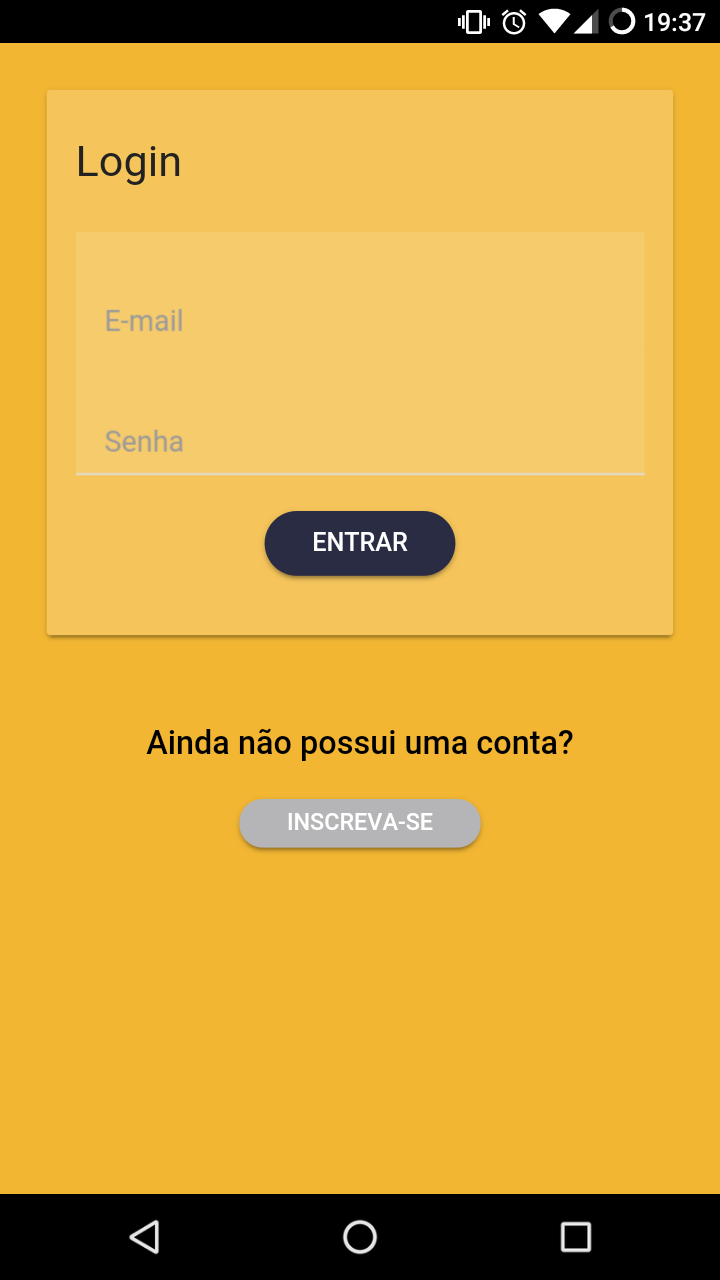
\includegraphics[scale=.55]{img/APP/login}}\qquad
    \subcaptionbox{\label{img:dados_atuais}Dados atuais}{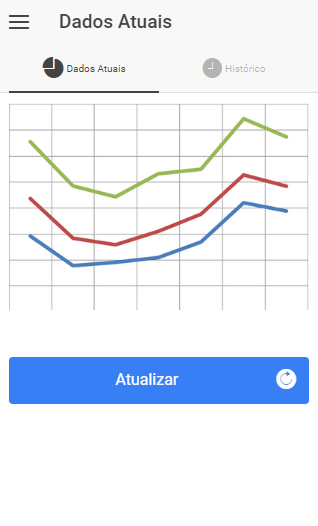
\includegraphics[scale=.55]{img/APP/dados_atuais}}\\
    \subcaptionbox{\label{img:hist-var}Escolher variáveis}{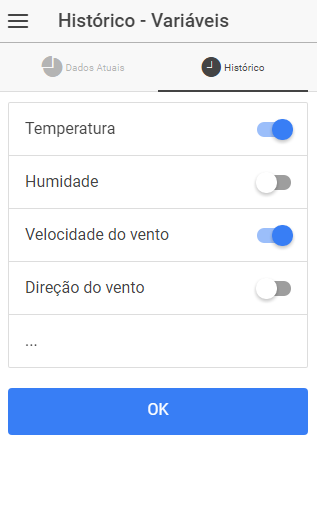
\includegraphics[scale=.55]{img/APP/hist-var}}\qquad
    \subcaptionbox{\label{img:hist-time}Seleção de período}{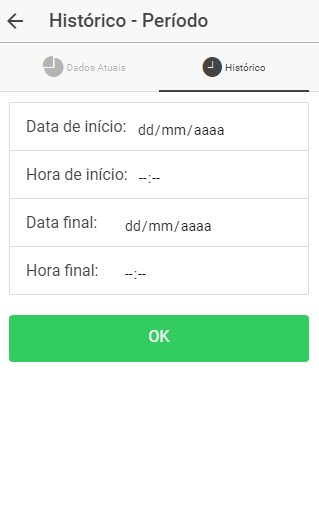
\includegraphics[scale=.55]{img/APP/hist-time}}\qquad
    \subcaptionbox{\label{img:hist-rel}Exibir histórico}{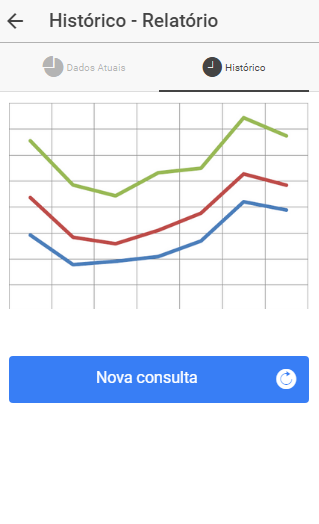
\includegraphics[scale=.55]{img/APP/hist-rel}}
    \legend{\textbf{Fonte:} O Autor}
\label{fig:dag}
\end{figure}

Além disso, será sempre permitido ao usuário retornar para a tela anterior através do botão voltar, com exceção da tela de \textit{login}, que só será acessível se o usuário realizar \textit{logoff} ou reiniciar a aplicação. O fluxo de funcionamento da aplicação cliente é representado pelo diagrama de atividades da figura \ref{img:atividades1} na subseção \ref{subsec:diagAtiv}.

A figura \ref{img:login} mostra a tela utilizada no caso de uso de autenticação do usuário. A figura \ref{img:dados_atuais} mostra a tela de visualização dos dados atuais. As figuras \ref{img:hist-var}, \ref{img:hist-time} e \ref{img:hist-rel} correspondem ao caso de uso de visualização de histórico.

É importante salientar que as telas aqui representadas são um protótipo, e durante a implementação do projeto podem sofrer alterações de \textit{design} e funcionalidades. Entretanto, já apresentam a ideia central de como será a aplicação.

\subsection{A API do sistema} \label{subsec:api}

Os URIs da API do sistema estão mostrados na tabela \ref{tab:api} abaixo. Assim como na subseção \ref{subsec:interfaceComOUsurario}, os identificadores aqui planejados são um protótipo e a medida que a implementação do sistema progride pode surgir a necessidade de alterá-los tanto sintaticamente quanto semânticamente. Assim como pode nascer a necessidade de adicionar novos identificadores ou de excluir algum dos planejados previamente.

A tabela divide-se em três partes, a primeira representa as ações que podem ser executadas por um usuário não autenticado, a segunda evidencia as ações possíveis para um usuário que efetuou \textit{login} e a terceira expõe as ações internas do sistema.

%\definecolor{Gray}{gray}{0.85}
\newpage

\begin{table}[!h]
\huge
\centering
\caption{\label{tab:api} API RESTful do sistema.}
\begin{adjustbox}{max width=\textwidth}
\begin{tabular}{@{} p{8.5cm} | l l p{10cm} @{}}
\toprule
%\rowcolor{Gray}
\multicolumn{1}{l}{Ator}                                 & Método & URI                                & Descrição                                                                                   \\ \hline
Usuário não autenticado              & POST   & /usuario/login                     & Autentica o usuário                                                                        ; \\ \hline
\multirow{5}{*}{Usuário autenticado} & GET    & /atual                             & Retorna o último documento da base de dados;                                                 \\ \cline{2-4}
                                     & GET    & /hist/\{id\_variavel\}/\{periodo\} & Retorna o histórico da variável no período especificado;                                     \\ \cline{2-4}
                                     & POST   & /usuario/novo                      & Cria um novo usuário com os parâmetros passados no corpo da requisição;                      \\ \cline{2-4}
                                     & PUT    & /usuario/\{username\}              & Atualiza os dados do usuário especificado com os parâmetros passados no corpo da requisição; \\ \cline{2-4}
                                     & DELETE & /usuario/\{username\}              & Deleta o usuário especificado;                                                               \\ \hline
\multirow{3}{*}{Sistema}             & POST   & /leitura                           & Cria um novo documento no banco os valores das variáveis passados no corpo da requisição;    \\ \cline{2-4}
                                     & DELETE & /leitura/\{id\}                    & Deleta a especificada leitura da base de dados;                                              \\ \cline{2-4}
                                     & PUT    & /leitura/\{id\}                    & Atualiza os dados da leitura especificada com os parâmetros passados no corpo da requisição; \\ %\cmidrule(l){2-4}
\bottomrule
                                      
\end{tabular}
\end{adjustbox}
\legend{\textbf{Fonte:} O Autor}
\end{table}





\subsection{Modelo de dados do sistema} \label{subsec:datamodel}

O banco de dados escolhido para a implementação do projeto é não-relacional baseado em documentos. Os documentos podem conter vários pares chave-valor, ou vários pares chave-vetor, ou até vários documentos encadeados. A estrutura do documento é flexível, o que permite alterações e inserções futuras de dados novos em uma base preexistente \cite{SITEMONGODB}. O modelo de dados inicial adotado para o projeto é mostrado na figura \ref{img:collection} abaixo, onde de um lado têm-se as chaves representando os dados fornecidos pela estação e do outro seus respectivos valores.

\imagem{0.55}{collection}{Modelo de documento do sistema}{O Autor}
\newpage

Os valores de cada chave adotada para o modelo de documentos são providos pelo \textit{datalogger} da estação. Algumas chaves possuem o valor obtido diretamente dos sensores, por exemplo a direção do vento. Em outros casos, os valores são calculados pela própria estação através de equações utilizando os dados derivados dos sensores, como por exemplo o ponto de orvalho, que faz uso da temperatura e da umidade externa em seu cálculo \cite{SITEVARIAVEIS}.

		\chapter{Conclusão e Trabalhos Futuros}

%Ao término das etapas apresentadas no cronograma da seção  espera-se obter um protótipo funcional de um sistema de monitoramento de variáveis meteorológicas cujos dados são provenientes de uma estação \textit{Vantage Vue™}, contendo todas as funcionalidades e características descritas no capítulo \ref{ch:MM}.

A preocupação em monitorar e prever as alterações climáticas do ambiente remete aos primórdios da humanidade. Com o passar do tempo e a consequente evolução da espécie, nos tornamos cada vez mais dependentes das condições do clima para garantir o sucesso no desenvolver de diversas atividades.

Neste trabalho foi elaborado e implementado um sistema de informação que coleta dados de uma estação meteorológica e a partir disso gera uma base de informações, permitindo consultas atuais e históricas das características medidas. As consultas são realizadas recorrendo à interface de usuário (\textit{Web / Android}) onde a \textit{internet} atua como meio de comunicação entre a base de dados e a aplicação cliente.

Compreende-se que os objetivos do trabalho foram atingidos de forma satisfatória. Pois, o protótipo dos sistema atendeu todos os requisitos propostos e mostrou resultados idênticos aos obtidos com o \textit{software} proprietário do fabricante da estação meteorológica em questão, no que diz respeito aos valores das variáveis climáticas.
 
\section{Trabalhos futuros}

Como trabalhos futuros pretende-se adicionar a funcionalidade ao sistema de monitorar os sensores da estação em tempo real, evitando necessidade do usuário agir e clicar em atualizar para verificar se há novos dados disponíveis.

Há também o objetivo de realizar a composição dos \textit{datasets} dos gráficos no servidor de aplicação (API), para então servi-los montados para a aplicação cliente,  melhorando assim a performance na exibição do histórico. 

Outro objetivo que se almeja é permitir monitorar diversas estações. A forma como o sistema foi implementado permite essa nova configuração com poucas linhas de código adicionais.

	\postextual
		\bibliography{tex/references_gabriel}
		\begin{anexosenv}
\chapter{Comandos seriais da estação meteorológica \textit{Vantage Vue™}} \label{anex:anexo1}

\begin{center}
\scalefont{0.85}
\begin{longtable}{ll}

\hline
\multicolumn{1}{c}{\textbf{Instrução}} & \multicolumn{1}{c}{\textbf{Descrição}} \\ \hline
\endfirsthead

\multicolumn{2}{c}%
{{\bfseries \tablename\ \thetable{} -- Continuação da página anterior}} \\

\hline
\multicolumn{1}{c}{\textbf{Instrução}} & \multicolumn{1}{c}{\textbf{Descrição}} \\ \hline
\endhead

\multicolumn{2}{r}{{Continua na próxima pagina}} \\
\endfoot

\endlastfoot

\multicolumn{2}{c}{\cellcolor{gray!25}\textbf{Comandos de teste}}                                                   		 \\ \hline
\textbf{TESTE}                            & Envia a \textit{string} "TEST\textbackslash n" de volta  \\ \hline
\textbf{WRD}                        & Responde com o tipo de estação meteorológica \\ \hline
\textbf{RXCHECK}                        & Responde com o diagnóstico do Console \\ \hline
\textbf{RXTEST}                       & Muda a tela do console de \textit{"Receiving from"} para tela de dados atuais                                                        \\ \hline
\textbf{VER}                           & Responde com a data do \textit{firmware}                                                             \\ \hline
\textbf{RECEIVERS}                    & Responde com a lista das estações que o console "enxerga" \\ \hline
\textbf{NVER}                       & Responde com a versão do \textit{firmware}                                                             \\ \hline
\multicolumn{2}{c}{\cellcolor{gray!25}\textbf{Comandos de dados atuais}}                                             \\ \hline
\textbf{LOOP}                     & Responde com a quantidade de pacotes especificada a cada 2s        \\ \hline
\textbf{LPS}                & Responde a cada 2s com a quantidade de pacotes diferentes especificada          \\ \hline
\textbf{HILOWS}                & Responde com todo os dados de \textit{high/low}                 \\ \hline
\textbf{PUTRAIN}                      & Seta a quantidade anual de precipitação \\ \hline
\textbf{PUTET}                 & Seta a quantidade anual de evapotranspiração        \\ \hline
\multicolumn{2}{c}{\cellcolor{gray!25}\textbf{Comandos de \textit{download}}}                                     		 \\ \hline
\textbf{DMP}                 & Faz o \textit{download} de todo o arquivo de memória \\ \hline
\textbf{DMAFT}                   & Faz o \textit{download} de todo o arquivo de memória após a data especificada \\ \hline
\multicolumn{2}{c}{\cellcolor{gray!25}\textbf{Comandos da EEPROM}}                                     		 \\ \hline
\textbf{GETEE}                 & Lê toda a memória EEPROM \\ \hline
\textbf{EEWR}                   & Escreve um \textit{byte} de dados à partir do endereço especificado                                   \\ \hline
\textbf{EERD}                   & Lê a quantidade de dados especificada iniciando no endereço especificado                                   \\ \hline
\textbf{EEBWR}                   & Escreve os dados na EEPROM                                    \\ \hline
\textbf{EEBRD}                   & Lê os dados da EEPROM \\ \hline
\multicolumn{2}{c}{\cellcolor{gray!25}\textbf{Comandos de calibração}}                                     		 \\ \hline
\textbf{CALED}                 & Envia os dados da temperatura e umidade corrente para atribuir à calibração \\ \hline
\textbf{CALFIX}                   & Atualiza o \textit{display} quando os números de calibração mudam\\ \hline
\textbf{BAR}                   & Seta os valores da elevação e o \textit{offset} do barômetro quando a localização é alterada                                   \\ \hline
\textbf{BARDATA}                   & Mostra os valores atuais da calibração do barômetro                                   \\ \hline \\
\multicolumn{2}{c}{\cellcolor{gray!25}\textbf{Comandos de limpeza}}                                     		 \\ \hline
\textbf{CLRLOG}                 & Limpa todo o arquivo de dados                                                       \\ \hline
\textbf{CLRALM}                   & Limpa todos os limiares dos alarmes                                   \\ \hline
\textbf{CLRCAL}                   & Limpa todos os \textit{offsets} da calibração da temperatura e da umidade \\ \hline
\textbf{CLRGRA}                   & Limpa o gráfico do console \\ \hline
\textbf{CLRVAR}                   & Limpa o valor da precipitação ou da evapotranspiração \\ \hline
\textbf{CLRHIGHS}                   & Limpa todos os valores de pico diários, mensais ou anuais                                   \\ \hline
\textbf{CLRLOWS}                   & Limpa todos os valores de mínimos diários, mensais ou anuais \\ \hline
\textbf{CLRBITS}                   & Limpa os \textit{bits} de alarme ativos                                  \\ \hline
\textbf{CLRDATA}                   & Limpa todos os dados atuais                                   \\ \hline
\multicolumn{2}{c}{\cellcolor{gray!25}\textbf{Comandos de configuração}}                                     		 \\ \hline
\textbf{BAUD}                 & Atribui o valor do \textit{baudrate} do console                                                       \\ \hline
\textbf{SETTIME}                   & Define a data e a hora do console                                   \\ \hline
\textbf{GAIN}                   & Define o ganho do receptor de rádio                                   \\ \hline
\textbf{GETTIME}                   & Retorna a hora e a data atual do console                                   \\ \hline
\textbf{SETPER}                   & Define o intervalo de arquivamento                                   \\ \hline
\textbf{STOP}                   & Desabilita a criação dos registros                                   \\ \hline
\textbf{START}                   & Habilita a criação dos arquivos \\ \hline
\textbf{NEWSETUP}                   & Reinicia o console após alguma configuração nova                                  \\ \hline
\textbf{LAMPS}                   & Liga ou desliga as lâmpadas do console \\ \hline
\caption{Comandos seriais suportados pela estação meteorológica \textit{Vantage Vue™}}
%\label{tab:6}
\end{longtable}
\fonte{\citeonline{VSPDOC} (Adaptado).}
\end{center}


\end{anexosenv}

\end{document}
